\documentclass[11pt]{article}
\usepackage{geometry}
\usepackage{amsmath}
\usepackage{pgfplots}
\pgfplotsset{compat=1.18}

\begin{document}
\pagestyle{empty}

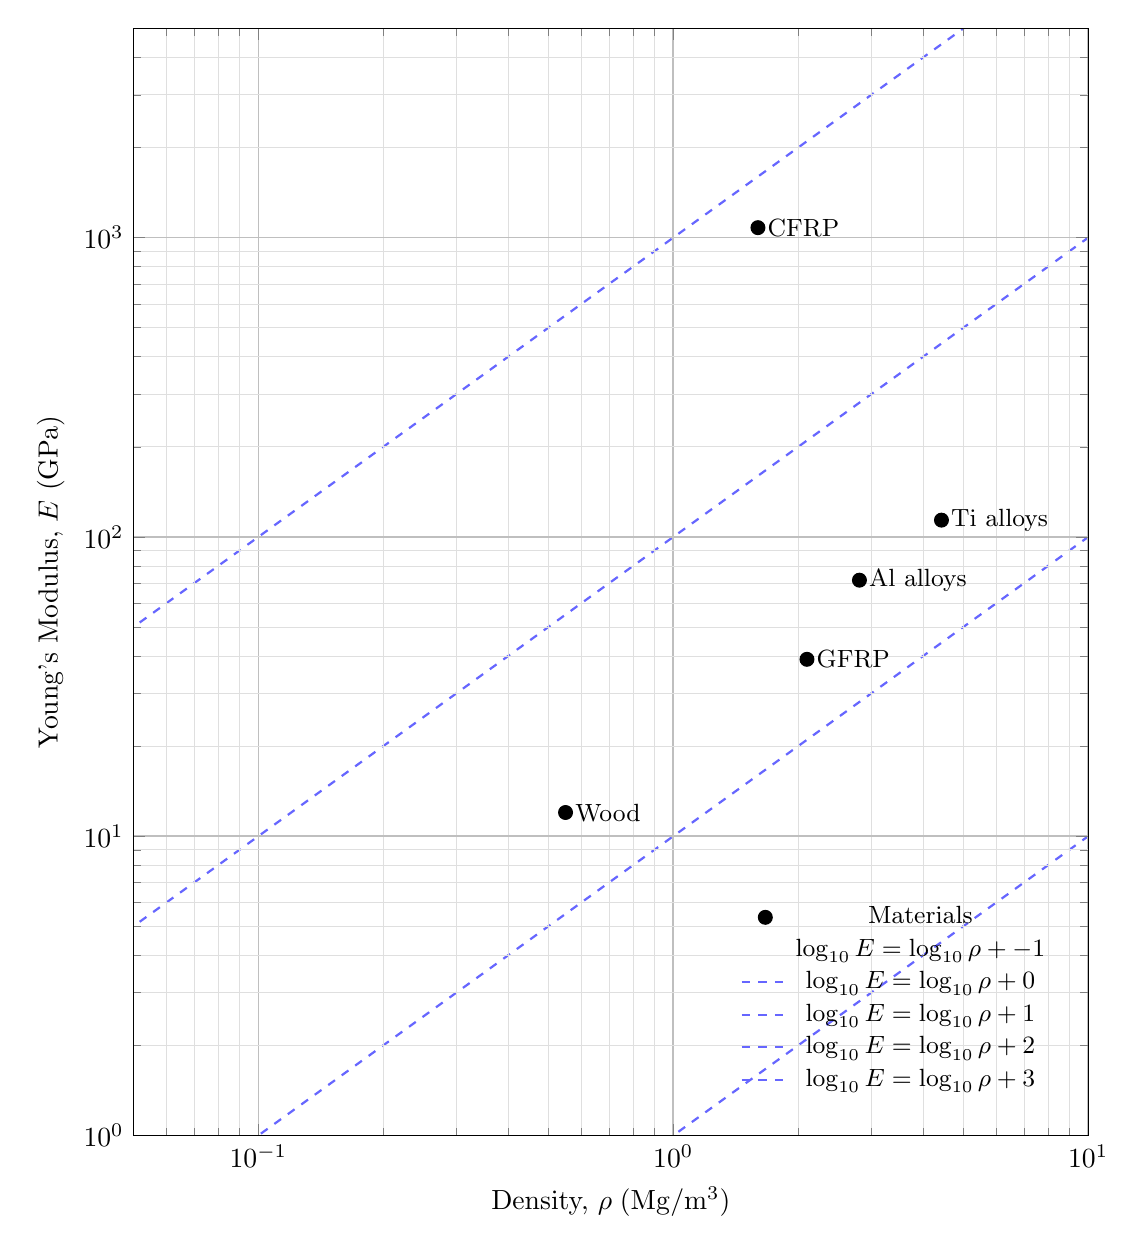
\begin{tikzpicture}
\begin{axis}[
  width=\textwidth, height=400pt, scale only axis,
  xmode=log, ymode=log,
  xmin=5e-2, xmax=1e1,
  ymin=1e0,  ymax=5e3,
  grid=both,
  major grid style={line width=0.6pt, draw=gray!50},
  minor grid style={line width=0.3pt, draw=gray!25},
  xlabel={Density, $\rho\;(\mathrm{Mg}/\mathrm{m}^{3})$},
  ylabel={Young's Modulus, $E$ (GPa)},
  legend style={draw=none, fill=none, font=\small},
  legend pos=south east,
  axis on top,
]

% numeric points
\addplot[only marks, mark=*, mark size=2.5pt, color=black] table {
x     y
0.550 12
4.430 113.8
2.810 71.7
2.100 39
1.600 1080
};
\addlegendentry{Materials}

% labels
\addplot[
  only marks, mark=none,
  nodes near coords,
  point meta=explicit symbolic,
  every node near coord/.style={anchor=west, font=\small}
] table[meta=label]{
x     y      label
0.550 12     {Wood}
4.430 113.8  {Ti alloys}
2.810 71.7   {Al alloys}
2.100 39     {GFRP}
1.600 1080   {CFRP}
};

% Lines: log10(E)=log10(rho)+C  =>  E = 10^C * rho
\pgfplotsinvokeforeach{-1,0,1,2,3}{
  \addplot[
    domain=1e-2:1e1, samples=2,
    dashed, thick, color=blue!60
  ] ({x},{(10^(#1))*x});
  \addlegendimage{no markers, dashed, thick, color=blue!60}
  \addlegendentry{$\log_{10}E=\log_{10}\rho + #1$}
}

\end{axis}
\end{tikzpicture}
\\
\newpage
Objective(Maximize): 
\\
\begin{align*}
 \text{Bending stiffnes per mass of material} &= \frac{EI}{m}; \text{    Where }m = \rho V
 \\
   &=\frac{EI}{\rho V}
    \\\text{This results in a material index M} &= \frac{E}{\rho}
    \\
    \log(M)&=\log(E) - log(\rho)
    \\
    \text{Material index loci in the form of: }  \log(E) &= \log(\rho) +\log(M)
\end{align*}


\end{document}